\documentclass[tikz,border=8pt]{standalone}
% Shared look for every TikZ diagram. Load with \input{../../tools/tikz-style.tex}
\usepackage[T1]{fontenc}
\usepackage{lmodern}
\renewcommand{\sfdefault}{lmr}  % diagrams use the same serif as the text
\usetikzlibrary{arrows.meta, positioning, shapes.geometric, calc, fit, backgrounds}
\definecolor{cblue}{HTML}{4C78A8}
\definecolor{corange}{HTML}{F58518}
\definecolor{cgreen}{HTML}{54A24B}
\definecolor{cred}{HTML}{E45756}
\definecolor{cpurple}{HTML}{B279A2}
\definecolor{cgrey}{HTML}{6B6B6B}
\tikzset{
  every picture/.style={font=\sffamily, line width=1.2pt},
  box/.style={draw=#1, fill=#1!12, rounded corners=4pt, align=center, inner sep=7pt, minimum height=1.1cm},
  box/.default=cgrey,
  arrow/.style={-{Stealth[length=3mm]}, draw=cgrey, line width=1.4pt},
  title/.style={font=\sffamily\bfseries\Large},
  note/.style={font=\sffamily\small, text=cgrey, align=center},
}
\AtBeginDocument{\hyphenpenalty=10000 \exhyphenpenalty=10000}

% Section 6: the chain from L back to W^1_11, one factor per link, with student 1's numbers.
% -7.36 x 0.1 x 8 = -5.888 (asserted in the Notebook and in Section 7.1).
\begin{document}
\begin{tikzpicture}[q/.style={box=#1, minimum width=1.9cm, minimum height=1.2cm, font=\Large},
                    back/.style={-{Stealth[length=3.5mm]}, draw=cred, line width=1.8pt},
                    f/.style={font=\large, align=center}]
  \node[q=cblue] (w) at (0, 0) {$W^{1}_{11}$};
  \node[q=corange] (o) at (5, 0) {$O_{11}$};
  \node[q=corange] (y) at (10, 0) {$\hat y$};
  \node[q=cred] (L) at (15, 0) {$L$};
  \draw[back] (L) -- node[f, above=4pt] {$\dfrac{\partial L}{\partial \hat y} = -2(y - \hat y)$} node[f, below=6pt, text=cred] {$-7.36$} (y);
  \draw[back] (y) -- node[f, above=4pt] {$\dfrac{\partial \hat y}{\partial O_{11}} = W^{2}_{11}$} node[f, below=6pt, text=cred] {$\times\ 0.1$} (o);
  \draw[back] (o) -- node[f, above=4pt] {$\dfrac{\partial O_{11}}{\partial W^{1}_{11}} = x_{i1}$} node[f, below=6pt, text=cred] {$\times\ 8$} (w);
  \node[f, font=\Large] at (7.5, -2.3)
    {$\dfrac{\partial L}{\partial W^{1}_{11}} = -7.36 \times 0.1 \times 8 = \mathbf{-5.888}$};
  \node[note, font=\large] at (7.5, -3.6) {first link shared by all 9 derivatives; an output weight stops after two links};
\end{tikzpicture}
\end{document}
